\chapter{Технологическая часть}
В данной части рассматривается выбор средств реализации, описывается структура классов программы и приводится интерфейс программного обеспечения.

Исходя из ролевой модели, представленной в предшествующих разделах создается ее реализация. 
Также предоставляется код для создания ролей, настройки их прав доступа и также создания триггера. 
Кроме того, предоставляется практический пример работы разработанного приложения.

\section{Выбор СУБД}

Самыми распространенными~\cite{sql-popular} СУБД реляционной модели БД являются:
\begin{itemize}
	\item PostgreSQL~\cite{postsql-db, sql-df};
	\item SQLite~\cite{sql-df};
	\item MySQL~\cite{sql-df}.
\end{itemize}

Выделим следующие критерии для сравнения полярных СУБД реляционной модели:
\begin{enumerate}
	\item возможность создавать роли, пользователей и выдавать им права доступа на уровне БД;
	\item активная поддержка;
	\item полное соответствие SQL.
\end{enumerate} 

В таблице~\ref{tbl:compare_DBMS} представлены результат сравнительного анализа популярных реляционных СУБД с учетом установленных критериев.

\begin{table}[ht!]
	\centering
	\caption{Сравнение популярных реляционных СУБД}
	\label{tbl:compare_DBMS}
	\begin{tabular}{|l|l|l|l|}
		\hline
		\textbf{Критерий} & \textbf{SQLite}& \textbf{MySQL} & \textbf{PostgreSQL}  \\ \hline
		
		Создания ролей & нет & есть & нет \\ \hline
		Поддержка & есть & нет & есть \\ \hline
		Соответствие SQL & нет & нет & есть  \\ \hline
		
	\end{tabular}
\end{table}

В данном работе выбрана PostgreSQL, поскольку она обеспечивает достаточный инструментарий для выполнения поставленной цели.

\section{Выбор средств реализации}

В качестве языка программирования для разработки программного обеспечения был применен язык C\#~\cite{csharp}, поскольку:
\begin{itemize}
	\item является объектно-ориентированным языком программирования, что позволяет создавать классы, объекты и методы, упрощая создания доступа к объектам базы данных и их взаимодействие связей;
	\item является частью платформы .Net~\cite{dotnet}, которая предоставляет необходимый набор библиотек и инструментов  для написания надежного и производительного программного продукта, работающего с различными базами данных;
	\item имеет встроенный механизм LINQ~\cite{linq}, который предоставляет возможности выполнения запросов к базе данных на уровне языка.
\end{itemize}

В качестве среда разработки был выбран Visual Studio~\cite{visualstudio}, так как:
\begin{itemize}
	\item данная среда разработки предоставляется бесплатно;
	\item поддерживает различный набор фреймворков NuGet~\cite{nuget};
	\item предоставляет интеграция управления версиями Git~\cite{git};
	\item мощные средства написания кода и функции --- все, что необходимо для создания приложений в одном месте;
	\item предоставляет шаблоны для создание и сборки проектов , что упрощает процесс разработки.
\end{itemize}

\section{Создание базы данных}

На листинге~\ref{dbcreate} представлено создание базы данных.

\begin{center}
	\begin{lstlisting}[label=dbcreate, caption=Создание базы данных]
CREATE DATABASE "PortalDb"
WITH
OWNER = postgres
ENCODING = 'UTF8'
LC_COLLATE = 'Russian_Russia.1251'
LC_CTYPE = 'Russian_Russia.1251'
TABLESPACE = pg_default
CONNECTION LIMIT = -1;
	\end{lstlisting}
\end{center}

На листингах~\ref{tablecreate-1}--\ref{tablecreate-5} представлено создание таблиц базы данных

\begin{center}
	\begin{lstlisting}[label=tablecreate-1, caption=Создание таблицы users]
CREATE TABLE IF NOT EXISTS public.users
(
	id uuid NOT NULL PRIMARY KEY,
	last_name varchar(64) NOT NULL,
	first_name varchar(64) NOT NULL,
	middle_name varchar(64),
	birthday timestamp with time zone NOT NULL,
	gender integer NOT NULL,
	email varchar(64) NOT NULL,
	phone varchar(64),
	password character varying(128) NOT NULL,
	role character varying(64) NOT NULL
);
	\end{lstlisting}
\end{center}

\clearpage

\begin{center}
	\begin{lstlisting}[label=tablecreate-2, caption=Создание таблиц zones inventories packages]		
CREATE TABLE IF NOT EXISTS public.zones
(
	id uuid NOT NULL PRIMARY KEY,
	name varchar(64) NOT NULL,
	address text NOT NULL,
	size double precision NOT NULL,
	"limit" integer NOT NULL,
	rating numeric NOT NULL
);

CREATE TABLE IF NOT EXISTS public.inventories
(
	id uuid NOT NULL PRIMARY KEY ,
	zone_id uuid NOT NULL 
	    REFERENCES public.zones (id) 
		MATCH SIMPLE
		ON UPDATE NO ACTION
		ON DELETE CASCADE,
	name varchar(64) NOT NULL,
	description text NOT NULL,
	date_production date NOT NULL,
	is_written_off boolean NOT NULL      
);

CREATE TABLE IF NOT EXISTS public.packages
(
	id uuid NOT NULL PRIMARY KEY,
	name varchar(64) NOT NULL,
	type varchar(64) NOT NULL,
	price numeric NOT NULL,
	rental_time integer NOT NULL,
	description text NOT NULL
);
	\end{lstlisting}
\end{center}

\clearpage

\begin{center}
	\begin{lstlisting}[label=tablecreate-3, caption=Создание ассоциативной таблицы zone\_packages и таблицы dishes]		
CREATE TABLE IF NOT EXISTS public.zone_packages
(
	package_id uuid NOT NULL
		REFERENCES public.zones (id) 
		MATCH SIMPLE
		ON UPDATE NO ACTION
		ON DELETE CASCADE,
	zone_id uuid NOT NULL 
		REFERENCES public.packages (id)
		MATCH SIMPLE
		ON UPDATE NO ACTION
		ON DELETE CASCADE,
	
	CONSTRAINT pk_zone_packages PRIMARY KEY (package_id, zone_id)
);

CREATE TABLE IF NOT EXISTS public.dishes
(
	id uuid NOT NULL PRIMARY KEY,
	name varchar(64) NOT NULL,
	type varchar(64) NOT NULL,
	price numeric NOT NULL,
	description text NOT NULL
);

	\end{lstlisting}
\end{center}

\clearpage

\begin{center}
	\begin{lstlisting}[label=tablecreate-4, caption=Создание ассоциативной таблицы package\_dishes и таблицы feedbacks]		
CREATE TABLE IF NOT EXISTS public.package_dishes
(
	dish_id uuid NOT NULL 
	REFERENCES public.dishes (id) 
	MATCH SIMPLE
	ON UPDATE NO ACTION
	ON DELETE CASCADE,
	package_id uuid NOT NULL
	REFERENCES public.packages (id) 
	MATCH SIMPLE
	ON UPDATE NO ACTION
	ON DELETE CASCADE,
	CONSTRAINT pk_package_dishes PRIMARY KEY (dish_id, package_id)
);

CREATE TABLE IF NOT EXISTS public.feedbacks
(
	id uuid NOT NULL PRIMARY KEY,
	user_id uuid NOT NULL
		REFERENCES public.users (id) 
		MATCH SIMPLE
		ON UPDATE NO ACTION
		ON DELETE CASCADE,
	zone_id uuid NOT NULL 
		REFERENCES public.zones (id) 
		MATCH SIMPLE
		ON UPDATE NO ACTION
		ON DELETE CASCADE,
	date timestamp with time zone NOT NULL,
	mark numeric NOT NULL,
	message text
);	
	\end{lstlisting}
\end{center}

\clearpage

\begin{center}
	\begin{lstlisting}[label=tablecreate-5, caption=Создание таблицы bookings]		
CREATE TABLE IF NOT EXISTS public.bookings
(
	id uuid NOT NULL PRIMARY KEY,
	zone_id uuid NOT NULL
		REFERENCES public.zones (id) 
		MATCH SIMPLE
		ON UPDATE NO ACTION
		ON DELETE CASCADE,
	user_id uuid NOT NULL
		REFERENCES public.users (id) 
		MATCH SIMPLE
		ON UPDATE NO ACTION
		ON DELETE CASCADE,
	package_id uuid NOT NULL
		REFERENCES public.packages (id) 
		MATCH SIMPLE
		ON UPDATE NO ACTION
		ON DELETE CASCADE,
	amount_of_people integer NOT NULL,
	status varchar(64) NOT NULL,
	date date NOT NULL,
	start_time time without time zone NOT NULL,
	end_time time without time zone NOT NULL,
	create_date_time timestamp with time zone NOT NULL,
	is_paid boolean NOT NULL,
	total_price numeric NOT NULL
);
	\end{lstlisting}
\end{center}

\clearpage

На листингах~\ref{rolecreate-1}--\ref{rolecreate-3} представлено создание ролей базы данных.

\begin{center}
	\begin{lstlisting}[label=rolecreate-1, caption=Создание ролей и выдача прав доступа (часть 1)]		
CREATE ROLE portal_admin WITH
SUPERUSER
CREATEDB
CREATEROLE
NOINHERIT
NOREPLICATION
NOBYPASSRLS
CONNECTION LIMIT -1
LOGIN
PASSWORD 'PaS$woRdAdm1N';

GRANT ALL PRIVILEGES 
ON ALL TABLES IN SCHEMA public 
TO portal_admin;

CREATE ROLE portal_user WITH
NOSUPERUSER
NOCREATEDB
NOCREATEROLE
NOINHERIT
NOREPLICATION
NOBYPASSRLS
CONNECTION LIMIT -1
LOGIN
PASSWORD 'PaS$woRdUser';

GRANT SELECT
ON ALL TABLES IN SCHEMA public 
TO portal_user;

	\end{lstlisting}
\end{center}

\clearpage

\begin{center}
\begin{lstlisting}[label=rolecreate-2, caption=Создание ролей и выдача прав доступа (часть 2)]
GRANT INSERT
ON public.users, 
public.bookings, 
public.feedbacks
TO portal_user; 

GRANT DELETE
ON public.bookings, 
public.feedbacks
TO portal_user;
	
GRANT UPDATE
ON public.bookings,
public.feedbacks
TO portal_user; 

CREATE ROLE portal_guest WITH
NOSUPERUSER
NOCREATEDB
NOCREATEROLE
NOINHERIT
NOREPLICATION
NOBYPASSRLS
CONNECTION LIMIT -1
LOGIN
PASSWORD 'PaS$woRdGuest';

	\end{lstlisting}
\end{center}

\clearpage

\begin{center}
	\begin{lstlisting}[label=rolecreate-3, caption=Создание ролей и выдача прав доступа (часть 3)]
GRANT SELECT
ON public.zones,
public.inventories,
public.feedbacks,
public.packages,
public.zonepackages,
public.dishes,
public.packagedishes
TO portal_guest;

GRANT INSERT
ON public.users
TO portal_guest;
	\end{lstlisting}
\end{center}

На листингах~\ref{triggercreate-1},~\ref{triggercreate-2}  представлено создание триггера после добавления записи в таблицу feedbacks на перерасчет рейтинга зоны антикафе по оставленным оценкам в отзыве пользователями.

\begin{center}
	\begin{lstlisting}[label=triggercreate-1, caption=Создание триггера (Часть 1)]
CREATE OR REPLACE FUNCTION public.calculate_rating_zone()
RETURNS TRIGGER
AS $$
BEGIN
	UPDATE public.zones
	SET rating = (Select sum(DISTINCT f.mark) / count(*) as rating 
				  from public.feedbacks as f
				   where f.zone_id = new.zone_id)
	WHERE id = new.zone_id;
RETURN NEW;
END;
$$ LANGUAGE PLPGSQL;
	\end{lstlisting}
\end{center}

\begin{center}
	\begin{lstlisting}[label=triggercreate-2, caption=Создание триггера (Часть 2)]
CREATE TRIGGER insert_feedbacks_trigger
AFTER INSERT ON public.feedbacks
FOR EACH ROW
EXECUTE FUNCTION public.calculate_rating_zone();
	\end{lstlisting}
\end{center}

\section{Интерфейс взаимодействия}

Для работы с базы данных был создан API с помощью библиотеки \\ Swashbuckle~\cite{swagger}. В программном интерфейсе реализованы методы для выполнения операций создания, чтения и удаления всех созданных сущностей в базе данных. На рисунках~\ref{fig:swagger-1}--\ref{fig:swagger-3} представлен методы интерфейса программы для взаимодействия с сущностями базы данных.

Методы взаимодействия с таблицей броней базы данных:
\begin{itemize}
	\item получение всех броней;
	\item получение брони по идентификатору;
	\item получение всех броней по идентификатору пользователя;
	\item получение всех броней по идентификатору зоны;
	\item создание брони;
	\item подтверждение брони;
	\item отмена брони.
\end{itemize}

Методы взаимодействия с таблицей отзывов базы данных:
\begin{itemize}
	\item получение всех отзывов;
	\item получение всех отзывов по идентификатору зоны;
	\item создание отзыва;
	\item удаление отзыва.
\end{itemize}

 Методы взаимодействия с таблицей инвентаря базы данных:
\begin{itemize}
	\item получение всего инвентаря;
	\item списать инвентарь зоны;
	\item создать и добавить инвентарь в зону.
\end{itemize}

Методы взаимодействия с таблицей блюд базы данных:
\begin{itemize}
	\item получение все блюда;
	\item получить блюда по идентификатору;
	\item создать блюдо;
	\item обновить данные блюда;
	\item удалить блюдо.
\end{itemize}

 Методы взаимодействия с таблицей пользователей базы данных:
\begin{itemize}
	\item зарегистрировать пользователя;
	\item авторизовать пользователя;
	\item получить дынные всех пользователей;
	\item получить данные пользователя по идентификатору.
\end{itemize}

 Методы взаимодействия с таблицей пакетов базы данных:
\begin{itemize}
	\item получить данные всех пакетов;
	\item получить данные пакета по идентификатору;
	\item создать пакет;
	\item обновить пакет;
	\item удалить пакет.
\end{itemize}

Методы взаимодействия с таблицей зон базы данных:
\begin{itemize}
	\item получить данные всех зон;
	\item получить данные зоны по идентификатору;
	\item создать зону;
	\item обновить зону;
	\item удалить зону.
\end{itemize}

\clearpage

\begin{figure}[h]
	\centering
	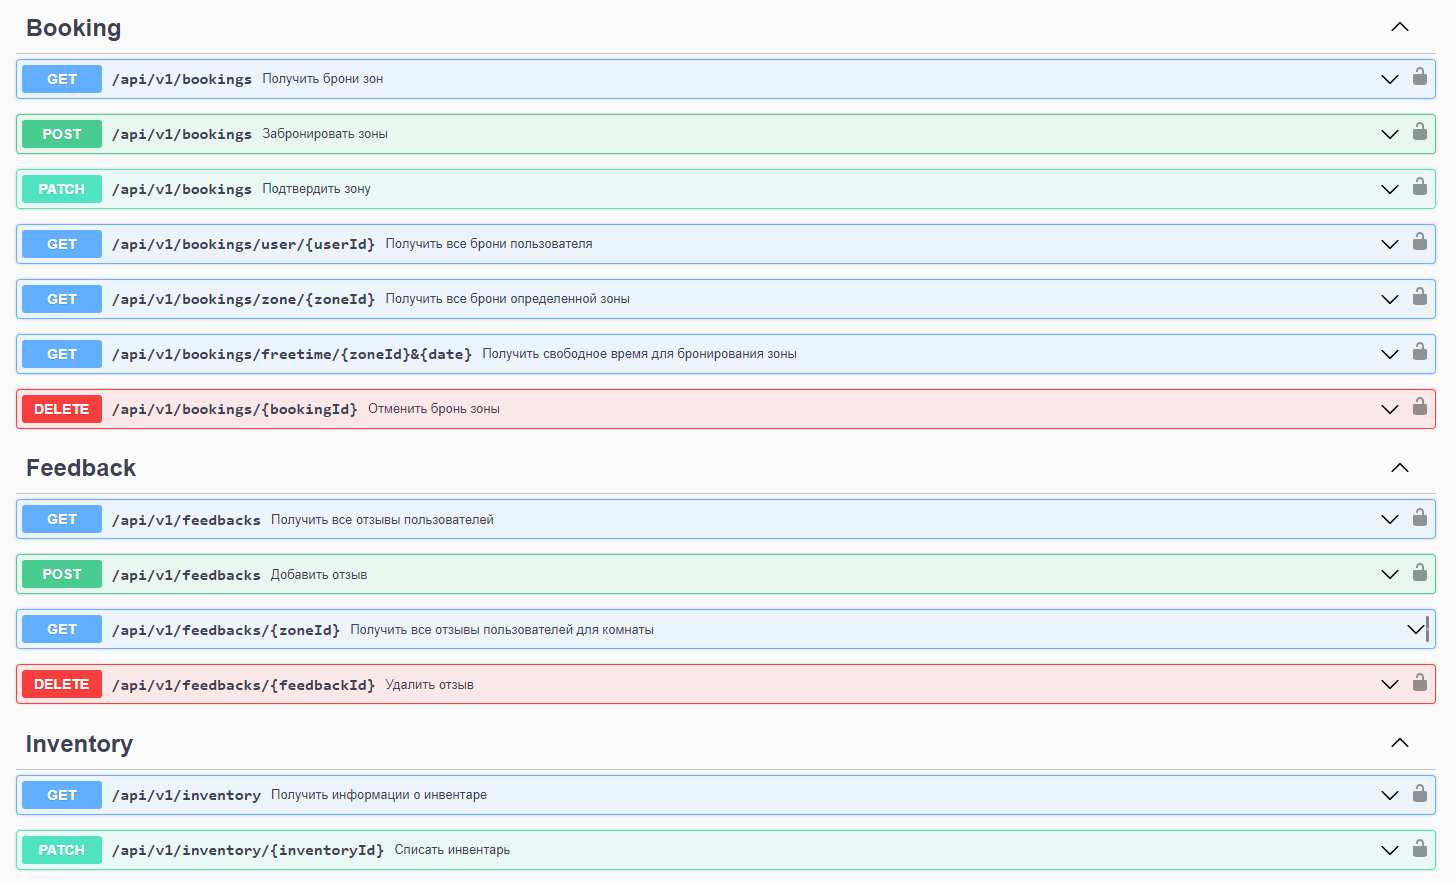
\includegraphics[height=0.3\textheight]{img/swagger-1.png}
	\caption{Программный интерфейс (часть 1)}
	\label{fig:swagger-1}
\end{figure}

\begin{figure}[h]
	\centering
	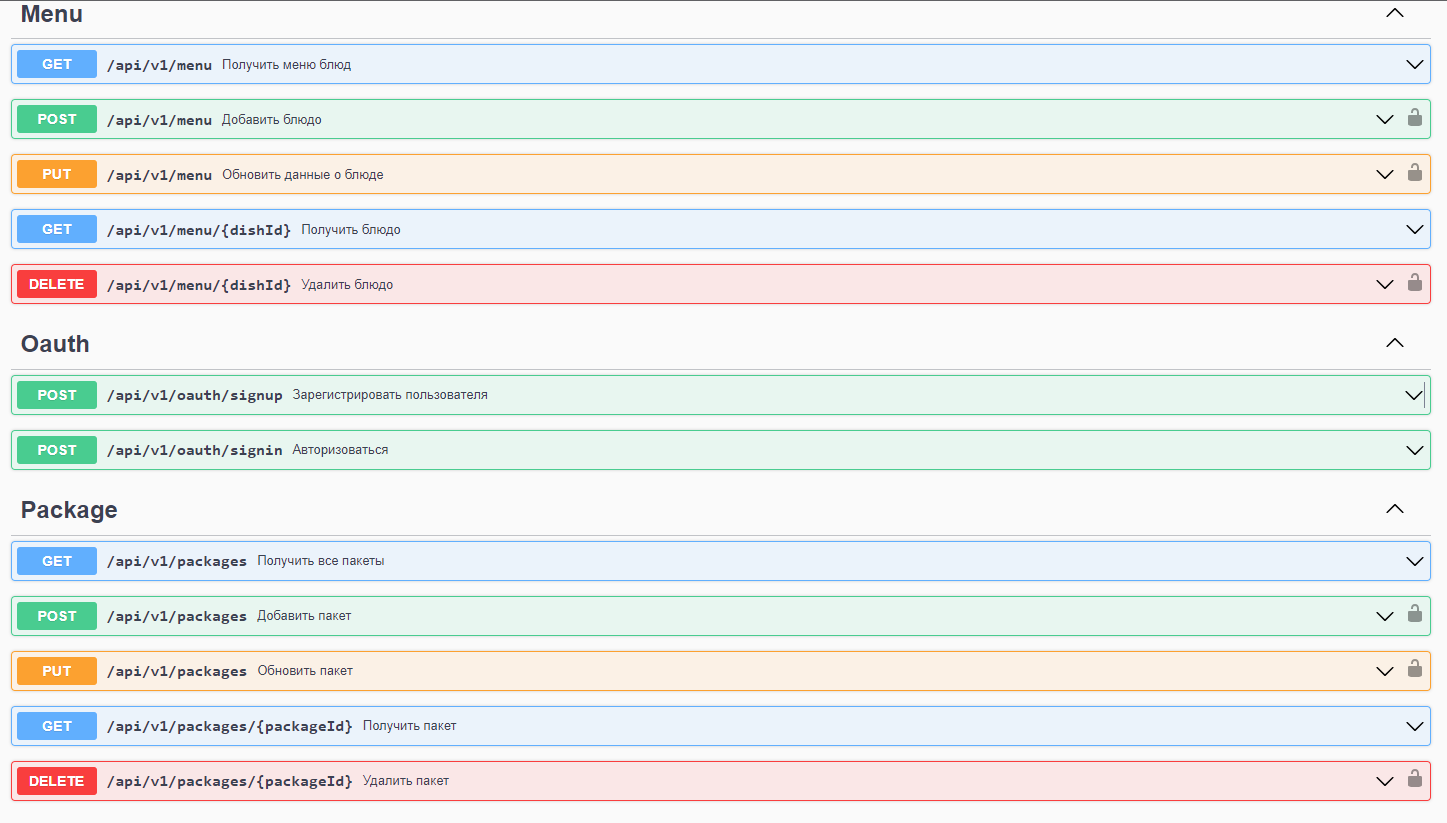
\includegraphics[height=0.3\textheight]{img/swagger-2.png}
	\caption{Программный интерфейс (часть 2)}
	\label{fig:swagger-2}
\end{figure}

\clearpage

\begin{figure}[h]
	\centering
	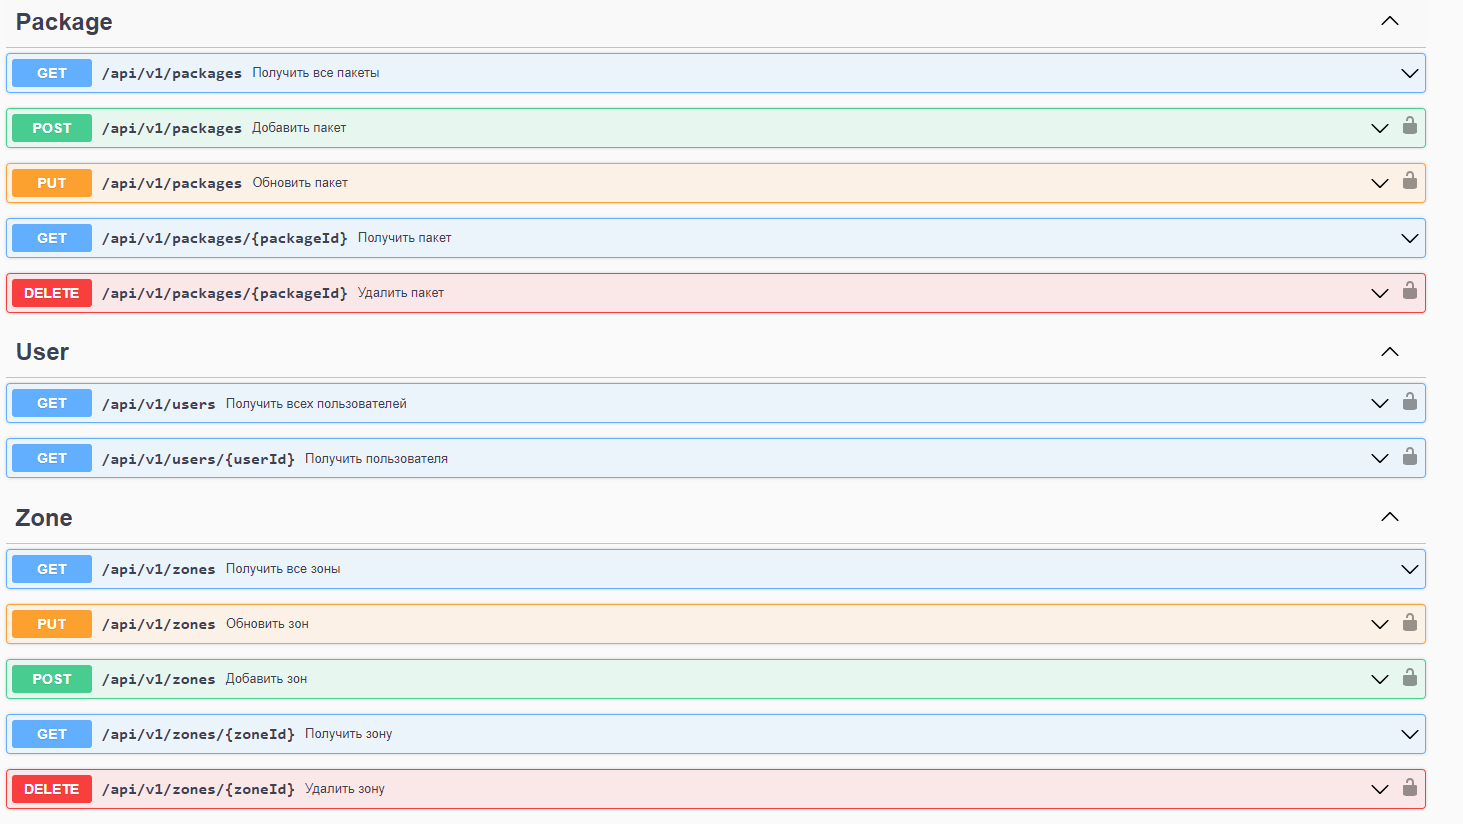
\includegraphics[height=0.3\textheight]{img/swagger-3.png}
	\caption{Программный интерфейс (часть 3)}
	\label{fig:swagger-3}
\end{figure}

\section{Демонстрация работы}

На рисунке~\ref{fig:example-1} показан процесс выполнения запроса, который направлен на получение всех доступных зон в базе данных. Этот запрос не предполагает наличие входных данных и возвращает JSON-объект с массивом данных о зонах. Информация о результатах запроса представлена в нижней части рисунке~\ref{fig:example-1}.

\clearpage

\begin{figure}[h]
	\centering
	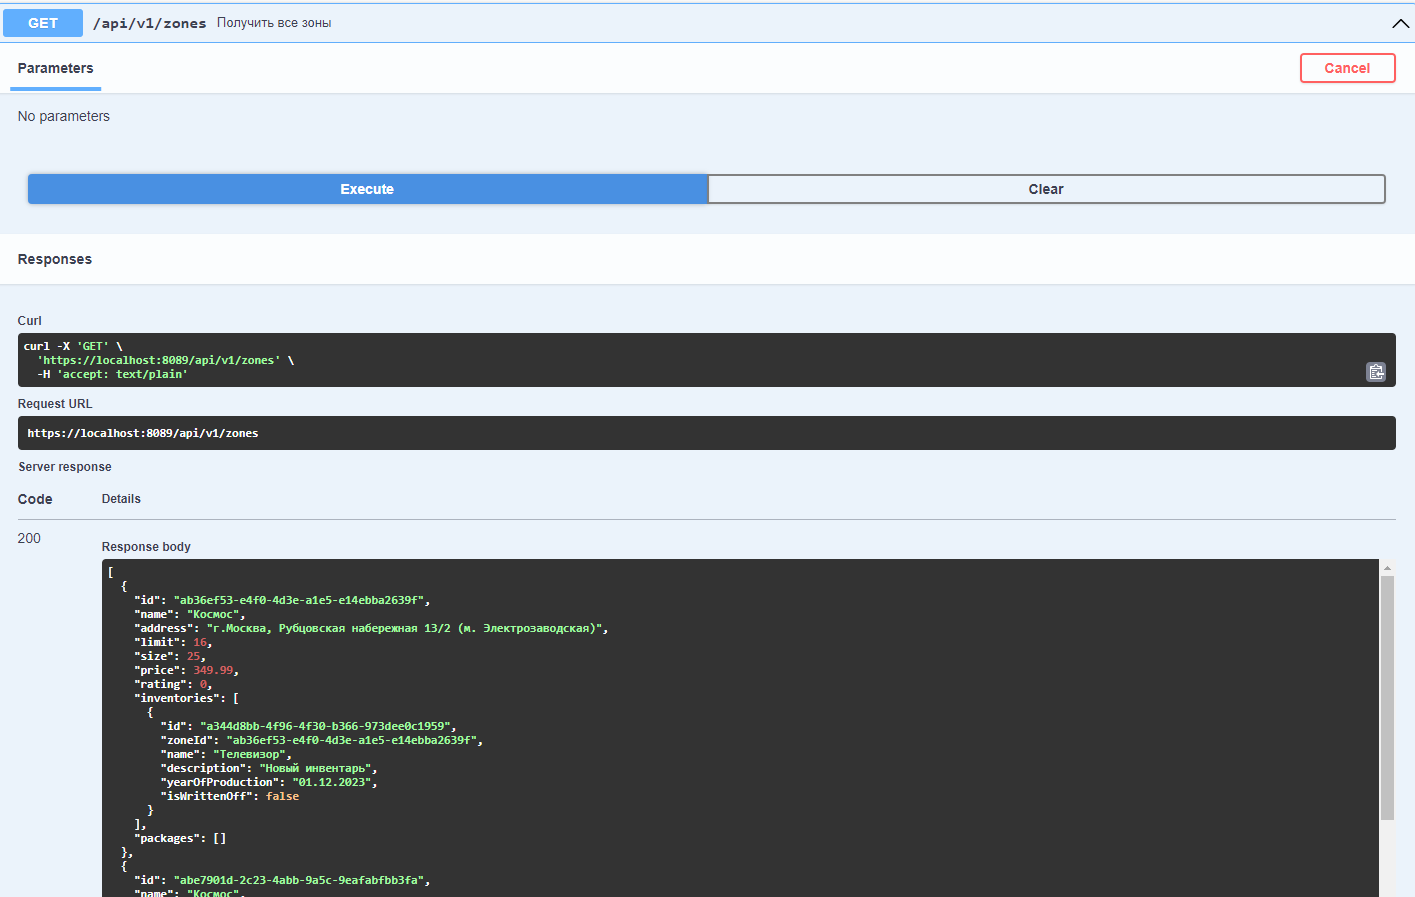
\includegraphics[height=0.35\textheight]{img/example-1.png}
	\caption{Демонстрация работы программы}
	\label{fig:example-1}
\end{figure}

\section*{Вывод}
В данном разделе была определена СУБД для работы с базой данных и средства реализации,  а также выполнены следующие задачи:  создание базы данных, таблиц, ролевой модели и триггера. Был описан разработанный пользовательский интерфейс и представлена демонстрация работы приложения. 